\documentclass[12pt]{article} % 12pt font size

% Packages
\usepackage[utf8]{inputenc}    % For UTF-8 character encoding
\usepackage[T1]{fontenc}       % For proper font encoding
\usepackage{lmodern}           % Improved font rendering
\usepackage{amsmath, amssymb}  % For math symbols and environments
\usepackage{graphicx}          % For including images
\usepackage{geometry}          % For adjusting page dimensions
\usepackage{hyperref}          % For clickable hyperlinks in the document
\usepackage{fancyhdr}          % For custom headers and footers
\usepackage{parskip}           % To add space between paragraphs
\usepackage{tikz}              % For drawing figures
\usepackage{booktabs}          % For improved table formatting
\usepackage{enumitem}          % For custom lists
\usepackage{caption}           % For customizing captions
\usepackage{listings}          % For code listings
\usepackage{multirow}          % For multirow tables
\usepackage{tikz}
\usetikzlibrary{automata, positioning}

\lstset{
  frame=tb,
  language=C,
  aboveskip=3mm,
  belowskip=3mm,
  showstringspaces=false,
  columns=flexible,
  basicstyle={\small\ttfamily},
  numbers=none,
  numberstyle=\tiny\color{gray},
  keywordstyle=\color{blue},
  commentstyle=\color{brown},
  stringstyle=\color{orange},
  breaklines=true,
  breakatwhitespace=true,
  tabsize=3
}

% Document settings
\geometry{margin=1in} % Set all margins to 1 inch

% Header and Footer customization
\pagestyle{fancy}
\fancyhf{}
\fancyhead[L]{\leftmark} % Left header contains the section name
\fancyhead[R]{\thepage}  % Right header contains the page number

\title{Document Title}
\author{WANG Xiyu}
\date{\today}

\begin{document}

\maketitle

\tableofcontents % Optional table of contents

\section{Introduction}
% Add your introduction here.

\section{$\epsilon$-Closure}
$\epsilon$-Closure of a state refers to the set of states where through n $\epsilon$ transitions (consuming n $\epsilon$ starting from the state by the NFA), that could be reached.\newline
Consider the below NFA, of which the transition function is listed as:

\begin{center}
    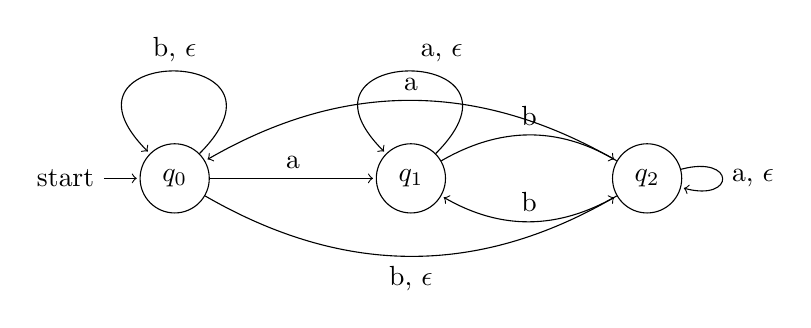
\begin{tikzpicture}[shorten >=1pt, node distance=3cm, on grid, auto]
        % Define the nodes
        \node[state, initial] (q_0) {$q_0$}; 
        \node[state] (q_1) [right=of q_0] {$q_1$}; 
        \node[state] (q_2) [right=of q_1] {$q_2$}; 
        % Define the transitions
        \path[->] 
        (q_0) edge[above] node {a} (q_1)
        (q_0) edge[bend right, below] node {b, $\epsilon$} (q_2)
        (q_0) edge[loop, above] node {b, $\epsilon$} (q_0)
        (q_1) edge[loop, above right] node {a, $\epsilon$} (q_1)
        (q_1) edge[bend left, above] node {b} (q_2)
        (q_2) edge[bend left, above] node {b} (q_1)
        (q_2) edge[bend right, above] node {a} (q_0)
        (q_2) edge[loop right, right] node {a, $\epsilon$} (q_2);
    \end{tikzpicture}
\end{center}
\[\delta(q_0, \epsilon ) = \{q_0, q_2\}\]
\[\delta(q_1, \epsilon ) = \{q_1\}\]
\[\delta(q_2, \epsilon ) = \{q_2\}\]
\[\delta(q_0, a) = \{q_1\}\]
\[\delta(q_0, b) = \{q_0, q_2\}\]
\[\delta(q_1, a) = \{q_1\}\]
\[\delta(q_1, b) = \{q_2\}\]
\[\delta(q_2, a) = \{q_0, q_2\}\]
\[\delta(q_2, b) = \{q_1\}\]
Thus the $\epsilon$-Closure of each state is:
\[EClose(q_0) = \{q_0, q_2\}\]
\[EClose(q_1) = \{q_1\}\]
\[EClose(q_2) = \{q_2\}\]



\subsection{Subsection Title}
% Add content for this subsection here.

\subsubsection{Subsubsection Title}
% Add content for this subsubsection here.

\begin{lstlisting}
    // Add your code example here
\end{lstlisting}

\begin{table}[h]
    \centering
    \begin{tabular}{|c|c|c|}
    \hline
    Column 1 & Column 2 & Column 3 \\ \hline
    Data 1 & Data 2 & Data 3 \\ \hline
    % Add more rows as needed
    \end{tabular}
    \caption{Table caption}
\end{table}

\begin{figure}[h]
    \centering
    \includegraphics[width=0.5\textwidth]{example-image} % Replace with your image file name
    \caption{This is a sample caption.}
    \label{fig:example}
\end{figure}

\end{document}
